\section{Tolkning av sannolikheter}
\par\bigskip
\noindent Om vi tar exemplet att singla slant. Vad betyder det att sannolikheten är $\dfrac{1}{2}$?\par
\noindent Man kan tolka det som att "det finns 2 fall, och båda har lika stor chans att inträffa"\par
\noindent Eller en mer data-inriktad tolkning, det vill säga om man singlar slant 100ggr, kommer ungefär hälften av kasten resultera i krona eller klave.
\par\bigskip
\noindent Det finns däremot tolkningar via Kolmogorovs axiom, det vill säga:
\begin{itemize}
  \item $P(A) = p$  betyder att $A$ utgör $p$ enheter av utfallsrummet $\Omega$
  \item Om vi upprepat slumpar ett $x\in\Omega$ så kommer tillslut $x\in A$  inträffa med frekvens $p$ (\textbf{stora talens lag})
\end{itemize}
\par\bigskip
\subsection{Sannolikhetsmåttet $P$}\hfill\\
\par\noindent Uppfyller följande:
\par\bigskip
\begin{itemize}
  \item $P(A^c) = 1-P(A)$
  \item $P(\O) = P(\Omega^c) = 1-P(\Omega) = 1-1 = 0$
  \item $A,B$ disjunkta gäller $P(A\cup B) = P(A\cup B \cup\O\cdots)$ (ty axiomet säger att vi skall ha oändliga disjunkta par, vi kan därför fylla ut med oändligt många tomma mängder) $\Rightarrow P(A)+P(B)$
  \item $P(B\setminus A) = P(B)-P(A\cap B)$
  \item Om $A\subseteq B$ så gäller $A\cap B = A$ och $P(B\setminus A) = P(B)-P(A)$
  \item Om $P(B\setminus A)\geq0$ så $A\subseteq B\Rightarrow P(A)\leq P(B)$
  \item $P(A\cup B) = P(A)+P(B)-\underbrace{P(A\cap B)}_{\text{$\geq0$}}$
  \item $P(A\cup B) \leq P(A)+P(B)$ (Booles olikhet)
\end{itemize}
\par\bigskip

\begin{theo}
  OOm $A_1\subseteq A_2\subseteq\cdots\subseteq\Omega$ så gäller
  \begin{equation*}
    \begin{gathered}
      P(\bigcup_{i=1}^{\infty}A_i) = \lim_{n\to\infty}P(A_n)
    \end{gathered}
  \end{equation*}
  \par\bigskip
  \noindent Kallas även för att sannolikhetsmåttet är kontinuerligt ovanifrån
\end{theo}
\par\bigskip
\begin{prf}[Bevis av föregående sats]{prf:prev}
  \begin{equation*}
    \begin{gathered}
      \underbrace{A_1}_{\text{$B_1$}}, \underbrace{A_2\setminus A_1}_{\text{$B_2$}},\underbrace{A_3\setminus A_2}_{\text{$B_3$}}\cdots \underbrace{A_{n+1}\setminus A_n}_{\text{$B_{n+1}$}}
    \end{gathered}
  \end{equation*}
  \par\bigskip
  \noindent $B_i$ är disjunkta, och följande gäller:
  \begin{equation*}
    \begin{gathered}
      \bigcup_{i=1}^{\infty}A_i = \bigcup_{i=1}^{\infty}B_i\\
      P\left(\bigcup_{i=1}^{\infty}A_i\right) = P\left(\bigcup_{i=1}^{\infty}B_i\right) = \sum_{i=1}^{\infty}P(B_i) = \lim_{n\to\infty}(P(B_1)+P(B_2)+P(B_3)+\cdots+P(B_n))\\
      \Lrarr \lim_{n\to\infty}(P(A_1)+(P(A_2)-P(A_1))+(P(A_3)-P(A_2))+\cdots+(P(A_n)-P(A_{n-1})))\\
      \Lrarr\lim_{n\to\infty}P(A_n)
    \end{gathered}
  \end{equation*}
\end{prf}
\newpage
\begin{theo}
  LLåt $A_3\subseteq A_2\subseteq A_1\cdots\subseteq\Omega$:
  \begin{equation*}
    \begin{gathered}
      P\left(\bigcap_{i=1}^{\infty}A_i\right) = \lim_{n\to\infty}P(A_n)
    \end{gathered}
  \end{equation*}
\end{theo}
\par\bigskip
\begin{lem}[De morgans lagar]{lem:demorgan}
  \begin{itemize}
    \item $\left(\bigcup_{i=1}^{\infty}A_i\right)^c = \bigcap_{i=1}^{\infty}A_i^c$
    \item $\left(\bigcap_{i=1}^{\infty}A_i\right)^c=\bigcup_{i=1}^{\infty}A_i^c$
  \end{itemize}
\end{lem}
\par\bigskip
\begin{prf}[Bevis av Lemma]{prf:lem}
  \begin{equation*}
    \begin{gathered}
      x\in\left(\bigcup_{i=1}^{\infty}A_i\right)^c\Lrarr x\notin \bigcup_{i=1}^{\infty}A_i\\
      \Lrarr x\notin A_i\quad \forall i\\
      \Lrarr x\in A_i^c\quad\forall i\\
      \Lrarr x\in\bigcap_{i=1}^{\infty}A_i^c
    \end{gathered}
  \end{equation*}
\end{prf}
\par\bigskip
\begin{prf}[Bebis av sats]{prf:prefv}
  Vi har $A_1^c\subseteq A_2^c\subseteq A_3^c\subseteq\cdots$:
  \begin{equation*}
    \begin{gathered}
      P\left(\bigcap_{i=1}^{\infty}A_i\right) = 1-P\left(\left(\bigcap_{i=1}^{\infty}A_i\right)^c\right) = 1-P\left(\bigcup_{i=1}^{\infty}A_i^c\right)\\
      \Rightarrow 1-\lim_{n\to\infty}P(A_i^c) = \lim_{n\to\infty}(1-P(A_i^c)) = \lim_{n\to\infty}P(A_n)
    \end{gathered}
  \end{equation*}
\end{prf}
\newpage
\section{Betingade sannolikheten $P(A|B)$}
\par\bigskip
\begin{theo}[Betingade sannolikheten]{thm:condprob}
  \begin{equation*}
    \begin{gathered}
      P(A|B) = \dfrac{P(A\cap B)}{P(B)} = \text{Sannolikheten för $A$ givet $B$ förutsatt att $P(B)>0$ och $P(A)>0$}
    \end{gathered}
  \end{equation*}\par
  \noindent Detta är sannolikheten att $x\in A$ givet att $x\in B$
\end{theo}
\par\bigskip
\noindent\textbf{Exempel:}
\par\bigskip
\noindent Låt $\Omega = \{1,2,3,4,\cdots\}$, $P(\{n\})=\dfrac{1}{2^n}$
\par\bigskip
\noindent Detta sade vi kunde representera antalet slantsinglingar som krävs för att landa på krona (eller klave)\par
\noindent Säg nu att vi sätter det här $B = $ första försöket landar på klave = $\{1\}^c = \{2,3,4,5,\cdots\}$
\par\bigskip
\noindent Vi förväntar oss att $P(1|B) = 0$ ($B$ gäller, alltså att vi har fått klave på första försöket, men då gäller det att det inte finns någon chans att vi får krona på första försöket)
\par\bigskip
\noindent Med motiveringen över gäller $P(2|B) = \dfrac{1}{2}$ och följande:
\begin{equation*}
  \begin{gathered}
    P(n|B) = \dfrac{1}{2^{n-1}} =\dfrac{P(\{n\}\cap B)}{P(B)} = \dfrac{P(\{n\})}{1/2} = 2P(n)=2\cdot\dfrac{1}{2^n} = \dfrac{1}{2^{n-1}}
  \end{gathered}
\end{equation*}
\par\bigskip
\noindent Vi kan definiera ett sannolikhetsmått $Q:2^B\to\R$ (för något $B\in\Omega$) och $Q(A) = \dfrac{P(A)}{P(B)}$ = betingade sannolikheten\par
\noindent Mer generellt kan vi definiera $Q:2^\Omega\to\R$ genom $Q(A) = \dfrac{P(A\cap B)}{P(B)}$ (med andra ord, den betingade sannolikheten)
\par\bigskip
\noindent För att visa att $Q$ är ett sannolikhetsmått måste vi visa att den uppfyller Kolmogorovs axiom:
\begin{itemize}
  \item $P(A)\geq0\quad \forall A\in2^{\Omega}$
  \item $P(\Omega) = 1$
  \item $P\left(\bigcup_{i=1}^{\infty}A_i\right) = \sum_{i=0}^{\infty}P(A_i)$ om $A_i$ är parvis disjunkta
\end{itemize}
\par\bigskip
\noindent Detta kommer inte vara så svårt, om vi visar det för $Q:2^\Omega\to\R$ så har vi visat det för $Q:2^B\to\R$.\par
\noindent\textbf{Vi visar första axiomet:} 
\begin{equation*}
  \begin{gathered}
    Q(A) = \dfrac{P(A\cap B)}{P(B)}\geq0\quad\forall A\in2^\Omega\\
  \end{gathered}
\end{equation*}
\par\bigskip
\noindent\textbf{Andra axiomet:} 
\begin{equation*}
  \begin{gathered}
  Q(\Omega) = \dfrac{P(\Omega\cap B)}{P(B)} = \dfrac{P(B)}{P(B)} = 1
  \end{gathered}
\end{equation*}
\par\bigskip
\noindent\textbf{Tredje axiomet:}\par
\noindent Antag $A_1, A_2,\cdots$ disjunkta. Då är $B\cap A_1, B\cap A_2,\cdots$ också disjunkta.\par
\noindent Vi vill räkna följande:
\begin{equation*}
  \begin{gathered}
    Q\left(\bigcup_{i=1}^{\infty}A_i\right) = \dfrac{P\left(\left(\bigcup_{i=1}^{\infty}A_i\right)\cap B\right)}{P(B)}
  \end{gathered}
\end{equation*}\par\bigskip
\noindent Notera:
\begin{equation*}
  \begin{gathered}
    \left(\bigcup_{i=1}^{\infty}A_i\right)\cap B = \bigcup_{i=1}^{\infty}(A_i\cap B)\text{ ty följande:}\\
    x\in \left(\bigcup_{i=1}^{\infty}A_i\right)\cap B\Rightarrow x\in A_i \text{ för något $i$ och $x\in B$}\\
    \Lrarr x\in A_i\cap B\text{ för något $i$}\\
    \Lrarr x\in \bigcup_{i=1}^{\infty}(A_i\cap B)
  \end{gathered}
\end{equation*}
\par\bigskip
\noindent Vi får då:
\begin{equation*}
  \begin{gathered}
    Q\left(\bigcup_{i=1}^{\infty}A_i\right) = \dfrac{P(\bigcup_{i=11}^{\infty}A_i\cap B)}{P(B)} = \dfrac{\sum_{i=1}^{\infty}P(A_i\cap B)}{P(B)} = \underbrace{\dfrac{\sum_{i=1}^{\infty}P(A_i\cap B)}{P(B)}}_{\text{$Q(A_i)$}} = \sum_{i=1}^{\infty}Q(A_i)
  \end{gathered}
\end{equation*}
\par\bigskip
\noindent Nu följer det till exempel att:
\begin{itemize}
  \item $P(A^c|B) = 1-P(A|B)$
  \item $P(A\cup C| B) = P(A|B)+P(C|B)-P(A\cap C |B)$
  \item Om $A\cap B\subseteq A_2\cap B\subseteq A_2\cap B\subseteq\cdots$ så gäller $P\left(\bigcup_{i=1}^{\infty}A_i|B\right) = \lim_{n\to\infty}P(A_n|B)$
\end{itemize}
\par\bigskip
\subsection{Oberoende utsagor}\hfill\\
\par
\noindent Antag att $P(A) >0$ och $P(B)>0$. Vi säger att $A$ och $B$ är \textbf{oberoende} om $P(A|B) = P(A)$ och $P(B|A) = P(B)$
\par\bigskip
\noindent\textbf{Anmärkning}:\par
\noindent $P(B|A) = P(B)\Lrarr P(A|B) = P(A)$. Kan bevisas genom Bayes sats.\par
\noindent Ytterliggare något att notera är att oberoende är ej en ekvivalensrelation ty den är ej transitiv.
\par\bigskip
\noindent\textbf{Exempel:}\par
\noindent Singla slant 2ggr, $\Omega = \{kr,kl\}^2$.\par
\noindent Vi ansätter $A= $ första försöket ger krona $= \{(kr,kr),(kr,kl)\}$\par
\noindent Vi ansätter $B = $ andra försöket ger krona $ = \{(kl,kr),(kr,kr)\}$
\par\bigskip
\noindent Vi får då följande:
\begin{equation*}
  \begin{gathered}
    P(A) = \dfrac{1}{2} = P(B)\qquad P(A\cap B) = P(kr,kr) = \dfrac{1}{4}\\\\
    P(A|B) = \dfrac{P(A\cap B)}{P(B)} = \dfrac{1/4}{1/2} = \dfrac{1}{2} = P(A)\\\\
    P(B|A) = \dfrac{P(B\cap A)}{P(A)} = \dfrac{1/4}{1/2} = \dfrac{1}{2}=P(B)\\\\
    \Rightarrow\text{$A$ och $B$ är oberoende}
  \end{gathered}
\end{equation*}
\par\bigskip
\noindent\textbf{Exempel:}\par
\noindent Låt $\Omega = $ Uppsalas vuxna befolkning.\par
\noindent Låt $A = \{\text{Man}\}\qquad B = \{\text{Bruna ögon}\}\qquad C = \{\text{Över 170cm}\}$
\par\bigskip
\noindent Avgör vilka som är oberoende
\newpage
\begin{theo}[Bayes sats]{thm:bais}

  \begin{equation*}
    \begin{gathered}
      P(B|A) = \dfrac{P(A|B)P(B)}{P(A)}
    \end{gathered}
  \end{equation*}
\end{theo}
\par\bigskip
\begin{prf}[Bays sats]{prf:bais}
  \begin{equation*}
    \begin{gathered}
      \dfrac{P(A|B)P(B)}{P(A)} = \dfrac{\dfrac{P(A\cap B)}{P(B)}P(B)}{P(A)} = \dfrac{P(A\cap B)}{P(A)} = P(B|A)
    \end{gathered}
  \end{equation*}
\end{prf}
\par\bigskip
\begin{theo}
  OOm $A\&B$ är oberoende så $\Lrarr A^c\&B$ oberoende $\Lrarr A\&B^c$ oberoende $\Lrarr A^c\&B^c$ oberoende
\end{theo}
\par\bigskip
\begin{prf}
  AAntag $A\&B$ är oberoende. Antag även att $P(A)>0, P(B)>0, P(A^c)>0, P(B^c)>0$$Q(A) = P(A|B)$ är ett sannolikhetsmått, då gäller:
  \begin{equation*}
    \begin{gathered}
      Q(A^c) = 1-Q(A)
    \end{gathered}
  \end{equation*}\par
  \noindent Det vill säga:
  \begin{equation*}
    \begin{gathered}
      P(A^c|B) = 1-\underbrace{P(A|B)}_{\text{$P(A)$}} = 1-(P(A)) = P(A^c)\Rightarrow A^c\&B\text{ är oberoende}
    \end{gathered}
  \end{equation*}\par
  \noindent Alla andra riktningar/implikationer följer på samma vis.
\end{prf}
\par\bigskip
\begin{theo}[Enkel liten sats]{thm:easypeasy}
  $A\&B$ är oberoende $\Lrarr P(A\cap B) = P(A)P(B)$
\end{theo}
\par\bigskip
\begin{prf}[Enkel liten sats]{prf:easypeasy}
  \begin{equation*}
    \begin{gathered}
      P(A|B) = P(A)\Lrarr \dfrac{P(A\cap B)}{P(B)} = P(A)\Lrarr P(A\cap B) = P(A)P(B)
    \end{gathered}
  \end{equation*}
\end{prf}
\par\bigskip
\begin{theo}[Oberoende (part 2)]{thm:independtwo}
  Detta är definitionen av oberoende vi i princip alltid kommer använda:\par
  \noindent $A$ och $B$ är oberoende om $P(A\cap B) = P(A)P(B)$
\end{theo}
\par\bigskip
\noindent\textbf{Anmärkning:}\par
\noindent Vad hännder om $P(A)$ eller $P(B)$ är 0?\par
\noindent Antag att $P(A) = 0$, eftersom $A\cap B\subseteq A\Rightarrow 0\leq P(A\cap B)\leq P(A) = 0$\par
\noindent Detta ger då att $P(A\cap B) = 0 = P(A\cap B) = 0\cdot P(B)$\par
\noindent Men då betyder det att $A$ och $B$ alltid är oberoende om $P(A) = 0$
\par\bigskip
\noindent\textbf{Anmärkning:}\par
\noindent Vad händer om $P(A) = 1$?\par
\noindent Rimligtvis borde $P(A\cap B) = 1\cdot P(B) = P(B)$. Detta sker:
\begin{equation*}
  \begin{gathered}
    A\subseteq A\cup B\Rightarrow 1 = P(A)\leq P(A\cup B)\leq 1\Rightarrow P(A\cup B) = 1\\
    \underbrace{P(A\cup B)}_{\text{1}} = \underbrace{P(A)}_{\text{1}}+P(B)-P(A\cap B)\\
    P(B)-P(A\cap B) = 0\Lrarr P(A\cap B) = P(B) = P(B)P(A)
  \end{gathered}
\end{equation*}
\par\bigskip
\noindent Om $P(A) = 1$ så är $A$ och $B$ alltid oberoende, alltså kan vi utöka Sats 4.3 till godtyckliga hänelser $A$ och $B$
\par\bigskip
\begin{theo}[Oberoende i flera variabler]{thm:multivariateindep}
  $S\subseteq 2^{\Omega}$ är obereonde om $A_1,\cdots, A_n\in S\Rightarrow P(A_1\cap\cdots\cap A_n) = P(A_1)\cdot\cdots\cdot P(A_n)$
\end{theo}
\par\bigskip
\noindent\textbf{Exempel:}\par
\noindent Säg att vi har en mängd $\left\{A,B,C\right\}$, mängden är obereonde om $P(A\cap B) = P(A)P(B)$ samt $P(A\cap C) = P(A)P(C)$ samt $P(B\cap C) = P(B)P(C)$ och $P(A\cap B\cap C) = P(A)P(B)P(C)$\par
\noindent Sista likheten är vitkig, ty om vi antar de 3 andra likheterna (parvis oberoende) är helt annat än full oberoende.
\par\bigskip
\noindent\textbf{Exempel:}\par
\noindent Låt $\Omega = \left\{1,2,3,4\right\}$, $P(n) = \dfrac{1}{4}$ samt $A = \left\{1,2\right\}$, $B=\left\{1,3\right\}$, $C = \left\{2,3\right\}$\par
\noindent Först och främst, $P(A) = \dfrac{1}{2} = P(B) = P(C)$\par
\noindent $P(A\cap B) = \dfrac{1}{4} = P(B\cap C) = P(A\cap C)\Rightarrow$ parvis oberoende\par
\noindent Om vi kollar sista grejen man måste kolla för obereonde, $P(A\cap\ B\cap C) = P(\O) = 0$, men $P(A)P(B)P(C) = \dfrac{1}{8}\neq0$, alltså ej oberoende i alla variabler.
\par\bigskip
\noindent\textbf{Anmärkning:}\par
\noindent Om $A,B,C$ är parvis oberoende så är inte $A,B,C$ nödvändigtvis oberoende, men om vi lägger till att $A$ och $B\cap C$ är oberoende, så är $A,B,C$ oberoende.\par
\noindent Detta gäller eftersom $P(A\cap(B\cap C)) = P(A)P(B\cap C) = P(A)P(B)P(C)$
\par\bigskip
\noindent\textbf{Exempel:}\par
\noindent Det är 22 personer i klassrummet, vad är sannolikheten att alla i klassrummet har olika födelsedagar? Vi kommer behöva göra några antaganden för att göra det här lite lättare för oss.\par
\noindent Vi betecknar $A_n = $ person $1,\cdots, n$ har olika födelsedagar. Det vi söker är $A_{22}$ (22 är en speciell siffra för det här problemet).\par
\noindent Antaganden:
\begin{itemize}
  \item Antag att $P(A_1) = 1$ (uppenbart att en person har samma födelsedag som en person)
  \item $P(A_{n+1}|A_n) = \dfrac{365-n}{365}$ lika stor sannolikhet att födas på alla dagar (inga skottår i vår miljö)
\end{itemize}\par
\noindent Notera, $A_{n+1}\subseteq A_n\Rightarrow A_n\cap A_{n+1} = A_{n+1}$ samt $P(A_{n+1}|A_n) = \dfrac{P(A_{n+1})}{P(A_n)}$
\par\bigskip
\noindent Vi har då $P(A_22) = P(A_{22}|A_{21})P(A_{21}) = P(A_{22}|A_{21})P(A_{21}|A_{20})P(A_{20}$\par
\noindent $= \cdots = \underbrace{P(A_{22}|A_{21})}_{\text{$\dfrac{344}{365}$}}\cdots = \dfrac{364!}{343!365^{21}} \approx 0.52$
\par\bigskip
\noindent Detta var för $P(A_{22})$, för $P(A_{n}) = \dfrac{364!}{(365-n)!365^{n-1}}$
\par\bigskip
\noindent Vi sade även att 22 var ett speciellt tal, detta ty $P(A_{23})\approx 0.49$, alltså där vi bryter 50 procent steget.
\par\bigskip
\noindent\textbf{Exempel:}\par
\noindent Antag att 80 procent av klassen gjorde inlämningsuppgifterna. Av de som gjorde inlämningsuppgifterna, så klarade 90 procent tentamen. Av de som inte gjorde inlämningsuppgifterna klarade 70 procent tentamen.\par
\begin{itemize}
  \item Hur stor andel klarade tentamen?
  \item Hur stor andel av de som klarade tentamen hade gjort inlämningsuppgifterna? 
\end{itemize}
\par\bigskip
\noindent Strategin här går ut på att skriva om uppgiften i matte-termer.\par
\noindent $\Omega =$ klassen, $A = $ de som gjorde inlämningsuppgifterna\par
\noindent $B =$ de som inte gjorde inlämningsuppgifterna $= A^c$\par
\noindent $C=$ de som klarade tentamen
\par\bigskip
\noindent Det vi har givet är att $P(A) = 0.8$, samt att $P(B) = =P(A^c) = 0.2$, $P(C|A) = 0.9$, $P(C^c|B) = 0.7 = P(C^c|A^c)$\par\bigskip
\noindent Vi söker $P(C)$. Vi vet även att $A\cup B$ samt att $A\cap B = \O$ (disjunkta).\par
\noindent Vi får då att $(A\cap C)\cup(B\cap C) = C$ samt $(A\cap C)\cap(B\cap C) = \O$\par
\noindent Vi skriver om $P(C) = P((C\cap A)\cup(C\cap B)) = \underbrace{P(A\cap C)}_{\text{$P(C|A)P(A)$}}+\underbrace{P(B\cap C)}_{\text{$P(C|B)P(B)$}}$\par
\noindent $\Rightarrow 0.9\cdot0.8+0.7\cdot0.2 = 0.86 = P(C)$
\par\bigskip
\noindent Nästa uppgift söker efter $P(A|C)$. Här kan vi använda Bayes sats:
\begin{equation*}
  \begin{gathered}
    P(A|C) = \dfrac{P(C|A)P(A)}{P(C)} = \dfrac{0.9\cdot0.9}{0.86} \approx 0.837
  \end{gathered}
\end{equation*}\par
\noindent Man kan tänka på det på följande sätt:
\begin{figure}[ht]
    \centering
    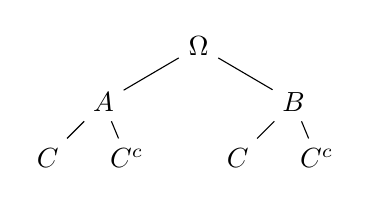
\begin{tikzpicture}
      \node (p0){$\Omega$};
      \node[below left of=p0, xshift=-.5cm](p1){$A$};
      \node[below right of=p0, xshift=.5cm](p2){$B$};
      \node[below left of=p1](p3){$C$};
      \node[right of=p3](p4){$C^c$};
      \node[below left of=p2](p5){$C$};
      \node[right of=p5](p6){$C^c$};
      \path (p0) edge (p1);
      \path (p0) edge (p2);
      \path (p1) edge (p3);
      \path (p1) edge (p4);
      \path (p2) edge (p5);
      \path (p2) edge (p6);
    \end{tikzpicture}
    \caption{}
\end{figure}
\par\bigskip
\noindent Från högstadiet kanske vi minns att om vi vill veta sannolikheten att $C-A-C$ och $C-B-C$ inträffar så multiplicerar vi $P(C)P(A)P(C)$ och adderar produkten $P(C)P(B)P(C)$, men detta är ju precis det vi har ägnat föreläsningen åt!\par
\begin{figure}[ht]
    \centering
    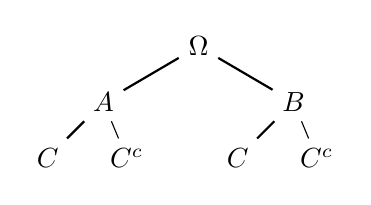
\begin{tikzpicture}
    \node (p0){$\Omega$};
      \node[below left of=p0, xshift=-.5cm](p1){$A$};
      \node[below right of=p0, xshift=.5cm](p2){$B$};
      \node[below left of=p1](p3){$C$};
      \node[right of=p3](p4){$C^c$};
      \node[below left of=p2](p5){$C$};
      \node[right of=p5](p6){$C^c$};
      \path[thick] (p0) edge (p1);
      \path[thick] (p0) edge (p2);
      \path[thick] (p1) edge (p3);
      \path (p1) edge (p4);
      \path[thick] (p2) edge (p5);
      \path (p2) edge (p6);
    \end{tikzpicture}
    \caption{}
\end{figure}
\begin{theo}[Lagen om total sannolikhet]{thm:law}
  Antag att $A_1,\cdots, A_n$ är disjunkta och $B\subseteq\bigcup_{i=1}^{n}$.\par
  \noindent Då är:
  \begin{equation*}
    \begin{gathered}
      P(B) = \sum_{i=1}^{n}P(B|A_i)P(A_i)
    \end{gathered}
  \end{equation*}\par\bigskip
  \noindent Specialfall: $A\cap A^c \Rightarrow P(B) = P(B|A)P(A)+P(B|A^c)P(A^c)$
\end{theo}
